\documentclass[12 pt]{article}
% Change "article" to "report" to get rid of page number on title page
\usepackage{amsmath,amsfonts,amsthm,amssymb}
\usepackage{setspace}
\usepackage{Tabbing}
\usepackage{fancyhdr}
\usepackage{lastpage}
\usepackage{extramarks}
\usepackage{chngpage}
\usepackage{indentfirst}
\usepackage{soul,color}
\usepackage{graphicx,float,wrapfig}
\usepackage{gauss}
\usepackage{dcolumn}
\newcolumntype{2}{D{.}{}{2.0}}
\usepackage{multicol}
\usepackage{Tabbing}
\usepackage{fancyhdr}
\usepackage{lastpage}
\usepackage{extramarks}
\usepackage{enumerate}
\usepackage{mathtools}
\usepackage{tikz}
\usetikzlibrary{positioning}
\usepackage{float}
\usepackage{wrapfig}



\graphicspath{ {/home/user/Documents/} }

\makeatletter
\renewcommand\section{\@startsection{section}{1}{\z@}%
                                  {-3.5ex \@plus -1ex \@minus -.2ex}%
                                  {2.3ex \@plus.2ex}%
                                  {\normalfont\bfseries}
                                }
\makeatother

\usepackage{etoolbox}
\makeatletter
\patchcmd\g@matrix
 {\vbox\bgroup}
 {\vbox\bgroup\normalbaselines}% restore the standard baselineskip
 {}{}
\makeatother

% In case you need to adjust margins:
\topmargin=-0.45in      %
\evensidemargin=0in     %
\oddsidemargin=0in      %
\textwidth=6.5in        %
\textheight=9.0in       %
\headsep=0.25in         %

% Homework Specific Information
\newcommand{\hmwkTitle}{$\S3.4$ Isomorphisms and $\S 3.5$ Cyclic Groups}
\newcommand{\hmwkDueDate}{Monday,\ October\ 26,\ 2015}
\newcommand{\hmwkClass}{Math\ 620}
\newcommand{\hmwkClassTime}{10:00}
\newcommand{\hmwkClassInstructor}{Boynton}
\newcommand{\hmwkAuthorName}{Kailee\ Gray}

\newtheorem{theorem}{Theorem}[section]
\newtheorem{lemma}[theorem]{Lemma}
\newtheorem{proposition}[theorem]{Proposition}
\newtheorem{corollary}[theorem]{Corollary}


\newenvironment{definition}[1][Definition]{\begin{trivlist}
\item[\hskip \labelsep {\bfseries #1}]}{\end{trivlist}}
\newenvironment{example}[1][Example]{\begin{trivlist}
\item[\hskip \labelsep {\bfseries #1}]}{\end{trivlist}}
\newenvironment{remark}[1][Remark]{\begin{trivlist}
\item[\hskip \labelsep {\bfseries #1}]}{\end{trivlist}}




% Setup the header and footer
\pagestyle{plain}                                                       %
\lhead{\hmwkAuthorName}                                                 %
\chead{\hmwkClass\ (\hmwkClassInstructor\ \hmwkClassTime): \hmwkTitle}  %
\rhead{\firstxmark}                                                     %
\lfoot{\lastxmark}                                                      %
\cfoot{}                                                                %
\rfoot{Page\ \thepage\ of\ \pageref{LastPage}}                          %
\renewcommand\headrulewidth{0.4pt}                                      %
\renewcommand\footrulewidth{0.4pt}                                      %

% This is used to trace down (pin point) problems
% in latexing a document:
%\tracingall

%%%%%%%%%%%%%%%%%%%%%%%%%%%%%%%%%%%%%%%%%%%%%%%%%%%%%%%%%%%%%
% Some tools
\newcommand{\enterProblemHeader}[1]{\nobreak\extramarks{#1}{#1 continued on next page\ldots}\nobreak%
                                    \nobreak\extramarks{#1 (continued)}{#1 continued on next page\ldots}\nobreak}%
\newcommand{\exitProblemHeader}[1]{\nobreak\extramarks{#1 (continued)}{#1 continued on next page\ldots}\nobreak%
                                   \nobreak\extramarks{#1}{}\nobreak}%

\newlength{\labelLength}
\newcommand{\labelAnswer}[2]
  {\settowidth{\labelLength}{#1}%
   \addtolength{\labelLength}{0in}%
   \changetext{}{-\labelLength}{}{}{}%
   \noindent\fbox{\begin{minipage}[c]{\columnwidth}#2\end{minipage}}%
   \marginpar{\fbox{#1}}%

   % We put the blank space above in order to make sure this
   % \marginpar gets correctly placed.
   \changetext{}{+\labelLength}{}{}{}}%

\setcounter{secnumdepth}{0}
\newcommand{\homeworkProblemName}{}%
\newcounter{homeworkProblemCounter}%
\newenvironment{homeworkProblem}[1][\arabic{homeworkProblemCounter}]%
  {\stepcounter{homeworkProblemCounter}%
   \renewcommand{\homeworkProblemName}{#1}%
   \section{\homeworkProblemName}%
   \noindent 
   
   \enterProblemHeader{\homeworkProblemName}}%
  {\exitProblemHeader{\homeworkProblemName}}%

\newcommand{\problemAnswer}[1]
  {\noindent\begin{minipage}[c]{\columnwidth}#1\end{minipage}}%

\newcommand{\problemLAnswer}[1]
    {\noindent\begin{minipage}[c]{\columnwidth}#1\end{minipage}}%

\newcommand{\homeworkSectionName}{}%
\newlength{\homeworkSectionLabelLength}{}%
\newenvironment{homeworkSection}[1]%
  {% We put this space here to make sure we're not connected to the above.
   % Otherwise the changetext can do funny things to the other margin

   \renewcommand{\homeworkSectionName}{#1}%
   \settowidth{\homeworkSectionLabelLength}{\homeworkSectionName}%
   \addtolength{\homeworkSectionLabelLength}{0 in}%
   \changetext{}{-\homeworkSectionLabelLength}{}{}{}%
   \subsection{\homeworkSectionName}%
   \enterProblemHeader{\homeworkProblemName\ [\homeworkSectionName]}}%
  {\enterProblemHeader{\homeworkProblemName}%

   % We put the blank space above in order to make sure this margin
   % change doesn't happen too soon (otherwise \sectionAnswer's can
   % get ugly about their \marginpar placement.
   \changetext{}{+\homeworkSectionLabelLength}{}{}{}}%

\newcommand{\sectionAnswer}[1]
  {\noindent\begin{minipage}[c]{\columnwidth}#1\end{minipage}}%
   \enterProblemHeader{\homeworkProblemName}\exitProblemHeader{\homeworkProblemName}%
  
 \newcommand{\R}{{\mathbb R}}
          \newcommand{\nil}{\varnothing}
          \newcommand{\N}{{\mathbb N}}
          \newcommand{\Z}{{\mathbb Z}}
        \newcommand{\MOD}{{ \ (\text{mod} \ }}

 \newcommand{\C}{{\mathbb C}}
  \newcommand{\Q}{{\mathbb Q}}
  
%%%%%%%%%%%%%%%%%%%%%%%%%%%%%%%%%%%%%%%%%%%%%%%%%%%%%%%%%%%%%
% Make title
\title{\vspace{2in}\textmd{\textbf{\hmwkClass:\ \hmwkTitle}}\\\normalsize\vspace{0.1in}\small{Due\ on\ \hmwkDueDate}\\\vspace{0.1in}\large{\textit{\hmwkClassInstructor\ \hmwkClassTime}}\vspace{3in}}
\date{}
\author{\textbf{\hmwkAuthorName}}
%%%%%%%%%%%%%%%%%%%%%%%%%%%%%%%%%%%%%%%%%%%%%%%%%%%%%%%%%%%%%

\begin{document}
\begin{spacing}{1.5}
\maketitle
 
% Uncomment the \tableofcontents and   lines to get a Contents page
% Uncomment the \setcounter line as well if you do NOT want subsections
%       listed in Contents
%\setcounter{tocdepth}{1}
%\tableofcontents
% 

% When problems are long, it may be desirable to put a   or a
% \clearpage before each homeworkProblem environment

\clearpage
\begin{flushleft}

\begin{homeworkProblem} [Exercise 3.4.10]
\textbf{Show that the group $\{f_{m,b}: \R \rightarrow \R \ |\  f(x)=mx+b, m\neq 0\}$ of affline functions from $\R$ to $\R$ (under composition of functions) is isomorphic to the group of all $2 \times 2$ matrices over $\R$ of the form $ M=  \left[\begin{array}{cc}
    m & b  \\
    0 & 1 
  \end{array} \right]$ with $m \neq 0$ (under matrix multiplication). }
\problemAnswer{ 
\begin{proof}
Let $A=\{f_{m,b}: \R \rightarrow \R \ |\  f(x)=mx+b, m\neq 0\}$	and let 
\[
F=\left\{B\in  M(2, \R) | \ B \text{ is of the form }   \left[\begin{array}{cc}
    m & b  \\
    0 & 1 
  \end{array} \right] \right\}. \text{ Define } \varphi: A \rightarrow F \text{ by } \varphi\left( f_{m,b} \right)= \left[\begin{array}{cc}
    m & b  \\
    0 & 1 
  \end{array} \right].
  \]
  \textbf{(one-to-one)} Consider $f_{a,b}$, $f_{c,d} \in A$ where $\varphi(f_{a,b})=\varphi(f_{c,d})$. Then, $\left[\begin{array}{cc}
    a & b  \\
    0 & 1 
  \end{array} \right] = \left[\begin{array}{cc}
    c & d  \\
    0 & 1 
  \end{array} \right]$ so $a=c$ and $b=d$. Therefore, $ax=cx$, so $ax+b=cx+d$. Thus, $f_{a,b}=f_{c,d}$.\\
  \\
  \textbf{(onto)} Let $\left[\begin{array}{cc}
    m & b  \\
    0 & 1 
  \end{array} \right] \in F$. Then, $f(x)=mx+b \in A$ and $\varphi(f(x))=\left[\begin{array}{cc}
    m & b  \\
    0 & 1 
  \end{array} \right]$. \\
  \\
  \textbf{(homomorphism)} Let $f_{a,b}$, $f_{c,d} \in A$ so $a, b, c, d \in \R$ and $a,c \neq 0$. Then,  $f_{a,b}\circ f_{c,d}=a(cx+d)+b=acx+ad+b$. 
  \[
  \text{So } \varphi(f_{a,b}\circ f_{c,d})=\varphi(f(x)=acx+ad+b)=\left[\begin{array}{cc}
    ac & ad+b  \\
    0 & 1 
  \end{array} \right] = \left[\begin{array}{cc}
    a & b  \\
    0 & 1 
  \end{array} \right] \left[\begin{array}{cc}
    c & d  \\
    0 & 1 
  \end{array} \right]=\varphi(f_{a,b})\varphi(f_{c,d})
  \]
  Thus, $\varphi$ is a group isomorphism from $A$ to $F$ which, by definition $3.4.1$, implies $A \cong F$.
\end{proof}

}
\end{homeworkProblem}

\begin{homeworkProblem}[Exercise 3.4.13: Let $C_2$ be the subgroup $\{\pm 1\}$ of the multiplicative group $\R^\times$. Show that $\R^\times$ is isomorphic to $\R^+ \times C_2$. ]
\problemAnswer{
Define $\varphi: \R^\times \rightarrow \R^{+}\times C_2$ by $\varphi(r)=(|r|, \frac{r}{|r|})$. Notice $|r|= r$ if $r>0$ and $|r|=-r$ if $r<0$, so $\frac{r}{|r|}=\pm 1 \in C_2$. Also, $|r|>0$ implies $|r| \in \R^{+}$ Since $r \in \R^\times$ implies $r \neq 0$, $\varphi$ is well defined. \\
\\
 \textbf{(one-to-one)} Consider $r_1, r_2 \in \R^\times$ where $\varphi(r_1)=\varphi(r_2)$. Then, $(|r_1|,\frac{r_1}{|r_1|})=(|r_2|, \frac{r_2}{|r_2|})$ so $|r_1|=|r_2|$ and $\frac{r_1}{|r_1|}=\frac{r_2}{|r_2|}$. $|r_1|=|r_2|$ implies $r_1=\pm r_2$. However, $\frac{r_1}{|r_1|}=\frac{r_2}{|r_2|}$ implies $\frac{r_1}{r_2}=\frac{|r_1|}{|r_2|}$ and so $\frac{r_1}{r_2}>0$. Thus, either $r_1>0$ and $r_2>0$ or $r_1<0$ and $r_2<0$. Suppose $r_1>0$ and $r_2>0$. Then, $|r_1|=r_1$ and $|r_2|=r_2$ so $r_1=r_2$. If $r_1<0$ and $r_2<0$, $|r_1|=-r_1$ and $|r_2|=-r_2$ so $-r_1=-r_2$ implies $r_1=r_2$. \\
  \\
  \textbf{(onto)} Consider $(r,c) \in \R^+\times C_2 $. Then, $r>0$ and $c=\pm 1$. First, consider $(r,1) \in \R^+\times C_2$. Then, for some $r \in \R^\times$ such that $r>0$, $\varphi(r)=(|r|, \frac{r}{|r|})=(r, \frac{r}{r})=(r, 1)\in \R^+ \times C_2$. Next, consider $(r,-1) \in \R^+\times C_2$. For some $r \in \R^\times$ such that $r<0$,  $\varphi(r)=(|r|, \frac{r}{|r|})=(-r, \frac{r}{-r})=(-r, -1)\in \R^+ \times C_2$.  \\
  \\
  \textbf{(homomorphism)} Let $r_1, r_2 \in \R^\times$ so $r_1, r_2 \neq 0$. Then,  $\varphi(r_1 r_2)=$
  \[
  \left(r_1r_2, \frac{r_1r_2}{|r_1r_2|}\right)=\left(r_1\cdot r_2, \frac{r_1r_2}{|r_1||r_2|}\right)= \left(r_1\cdot r_2, \frac{r_1}{|r_1|}\cdot\frac{r_2}{|r_2|}\right)=\left(r_1, \frac{r_1}{|r_1|}\right)\cdot \left(r_2, \frac{r_2}{|r_2|}\right)=\varphi(r_1)\varphi(r_2).
  \] 
  \\
 Thus, $\varphi$ defines a group isomorphism from $\R^\times$ to $\R^+\times C_2$ which, by definition $3.4.1$, implies $\R^\times \cong \R^+\times C_2$.
}
\end{homeworkProblem}
 \newpage
\begin{homeworkProblem}[Exercise 3.4.15: Let $G$ be any group, and let $a$ be a fixed element of $G$. Define a function $\phi_a:G \rightarrow G$ by $\phi_a(x)=axa^{-1}$ for all $x \in G$. Show that $\phi_a$ is an isomorphism.]
 \begin{proof}
 Let $G$ be any group, and let $a$ be a fixed element of $G$. Define a function $\phi_a:G \rightarrow G$ by $\phi_a(x)=axa^{-1}$ for all $x \in G$.\\
 \textbf{(one-to-one)} Consider $x_1, x_2 \in G$ where $\phi(x_1)=\phi(x_2)$. Then, $ax_1 a^{-1}=ax_2a^{-1}$. Notice 
  \[\begin{array}{lll}
	ax_1 a^{-1}a& =ax_2a^{-1}a & \text{multiply on the right by } a \\
	ax_1e & =ax_2e &  \text{ because } a^{-1}a=e, \text{ the identity element in } G\\
	a^{-1}ax_1 & =a^{-1}ax_2 &  \text{ because } x_1e=x_1 \text{ and } x_2e=x_2\text{. Then, multiply on the left by } a^{-1}\\
	ex_1 & =ex_2 &  \text{ because } a^{-1}a=e \\
	x_1 & =x_2 &  \text{ because } ex_1=x_1 \text{ and } ex_2=x_2\\
\end{array}
 \]
\\
  \textbf{(onto)} Consider $x_1 \in G$. Then, $a, a^{-1} \in G$ implies $a^{-1}x_1a \in G$, so
  \[\begin{array}{lll}
  \phi(a^{-1}x_1a)&=a(a^{-1}x_1a)a^{-1}& \text{ by definition of } \phi \\
   &=(aa^{-1})x_1(aa^{-1})& \text{ $G$ is a group so the operation of $G$ is associative } \\
     &=(e)x_1(e)& \text{ because } aa^{-1}=e \\
      &=(ex_1)(e)& \text{ $G$ is a group so the operation of $G$ is associative } \\
      &=x_1& \text{ definition of the identity element} \\
  \end{array}
  \]
    \textbf{(homomorphism)} Let $x_1, x_2 \in G$. Then, by the associative law of $G$ and the definition of the identity element and inverses in $G$ we have, 
  \[
  \phi(x_1 x_2)=a(x_1x_2)a^{-1}=a(x_1ex_2)a^{-1}=a(x_1(a^{-1}a)x_2)a^{-1}=(ax_1a^{-1})(ax_2a^{-1})=\phi(x_1)\phi(x_2).
  \] 
 Thus, $\phi$ defines a group isomorphism from $G$ to $G$.
 \end{proof}
 
\end{homeworkProblem}
 
\begin{homeworkProblem}[Exercise 3.4.16: Let $G$ be any group. Define $\phi: G \rightarrow G$ by $\phi(x)=x^{-1}$, for all $x \in G$.]
\textbf{(a) Prove that $\phi$ is one-to-one and onto.}
\begin{proof}
\textbf{(one-to-one)} Consider $x_1, x_2 \in G$ and suppose $\phi(x_1)=\phi(x_2)$. Then, $x_1^{-1}=x_2^{-1}$. Since $x_1^{-1}, x_2^{-1} \in G$, $x_1^{-1},x_2^{-1}$ have inverses in $G$, so $(x_1^{-1})^{-1}=(x_2^{-1})^{-1}$. Thus, $x_1=x_2$.
\textbf{(onto)} Let $x \in G$. Then, $x^{-1} \in G$ and $\phi(x^{-1})=(x^{-1})^{-1}=x$.
\end{proof}
\textbf{(b) Prove that $\phi$ is an isomorphism if and only if $G$ is abelian.}
\begin{proof}
$(\Rightarrow)$ Assume $\phi$ is an isomorphism. Then, $\phi$ is a homomorphism, so for any $x_1, x_2$, $\phi(x_1x_2)=\phi(x_1)\phi(x_2)$. Since $\phi(x_1x_2)=(x_1x_2)^{-1}=x_2^{-1}x_1^{-1}$ and $\phi(x_1)\phi(x_2)=x_1^{-1}x_2^{-1}$. Thus, $x_2^{-1}x_1^{-1}=x_1^{-1}x_2^{-1}$ implies $(x_2^{-1}x_1^{-1})^{-1}=(x_1^{-1}x_2^{-1})^{-1}$. Further, $(x_1^{-1})^{-1}(x_2^{-1})^{-1}=(x_2^{-1})^{-1}(x_1^{-1})^{-1}$. Equivalently, $x_1x_2=x_2x_1$. Thus, $G$ is abelian.\\
$(\Leftarrow)$ Assume $G$ is abelian. Then, for any $x_1,x_2 \in G$, $x_1x_2=x_2x_1$. We can follow our previous argument backwards to obtain
\[
\begin{array}{ll}
x_1x_2 & =x_2x_1\\
(x_1^{-1})^{-1}(x_2^{-1})^{-1}& =(x_2^{-1})^{-1}(x_1^{-1})^{-1}\\
(x_2^{-1}x_1^{-1})^{-1} & =(x_1^{-1}x_2^{-1})^{-1} \\
x_2^{-1}x_1^{-1} & =x_1^{-1}x_2^{-1}\\
(x_1x_2)^{-1} & = \phi(x_1)\phi(x_2)\\
\phi(x_1x_2) & = \phi(x_1)\phi(x_2)\\
\end{array}
\]
Thus, $\phi$ is a homomorphism. From part (a), we know $\phi$ is one-to-one and onto. Thus, $\phi$ is an isomorphism. 
\end{proof}

\end{homeworkProblem}

\begin{homeworkProblem}[Exercise 3.4.22: Let $a,b$ be positive integers, and let gcd$(a,b)=d$ and $m=\text{lcm}\lbrack a,b \rbrack$. Write $d=sa+tb$, $a=a'd$, and $b=b'd$. Prove that the function $f:\Z_m\times\Z_d \rightarrow \Z_a \times \Z_b$ defined by $f((\lbrack x \rbrack _m,\lbrack y \rbrack _d))=(\lbrack x+ysa' \rbrack_a,\lbrack x-ytb' \rbrack)_b$ is an isomorphism. ] 
\begin{proof}
 \textbf{(well-defined)} Suppose there exists elements in $\Z_m \times \Z_d$ such that $(\lbrack x_1 \rbrack _m,\lbrack y_1 \rbrack _d)=(\lbrack x_2 \rbrack _m,\lbrack y_2 \rbrack _d)$. Then, 
 \begin{equation}
 x_1 \equiv x_2 \MOD m) \text{ and } y_1 \equiv y_2 \MOD d). 
 \end{equation}
\begin{equation}
\text{ Equivalently, for some } l, k \in \Z, \  \ x_1=x_2 + lm \text{ and } y_1 = y_2 + kd	
\end{equation}
Since $a | m$, we can write (2) as $x_1=x_2+ll'a$ for some $l' \in \Z$. Thus, $x_1 \equiv x_2 \MOD a)$. Also from (2), we can multiply by $a'$ to obtain $a'y_1=a'y_2+a'kd$ which, because $a'd = a$, we can write $a'y_1=a'y_2+ka$. Multiplying by $s$, we have $sa'y_1=sa'y_2+ska$; equivalently $sa'y_1 \equiv sa'y_2 \MOD a)$. Thus, since $x_1 \equiv x_2 \MOD a)$ and $sa'y_1 \equiv sa'y_2 \MOD a)$, we have
\begin{equation}
	x_1+sa'y_1 \equiv x_2+sa'y_2 \MOD a )
\end{equation}
Similarly, since $b|m$, we can write (2) as $x_1=x_2+ll^{''}b$ for some $l^{''} \in \Z$. Thus, $x_1 \equiv x_2 \MOD b)$. Also from (2), we can multiply by $b'$ to obtain $b'y_1=b'y_2+b'kd$ which, because $b'd = b$, we can write $b'y_1=b'y_2+kb$. Multiplying by $-t$, we have $-tb'y_1=-tb'y_2-tkb$; equivalently $-tb'y_1 \equiv -tb'y_2 \MOD b)$. Thus, since $x_1 \equiv x_2 \MOD b)$ and $-tb'y_1 \equiv -tb'y_2 \MOD b)$, we have
\begin{equation}
	x_1-tb'y_1  \equiv x_2  -tb'y_2  \MOD b )
\end{equation}
Equations (3) and (4) imply $f((\lbrack x_1 \rbrack _m,\lbrack y_1 \rbrack _d))=f((\lbrack x_2 \rbrack _m,\lbrack y_2 \rbrack _d))$.
\\
\textbf{(homomorphism)} Consider any $(\lbrack x_1 \rbrack _m,\lbrack y_1 \rbrack_d), (\lbrack x_2 \rbrack _m,\lbrack y_2 \rbrack _d)$ in $\Z_m \times \Z_d$.  Then, $(\lbrack x_1 \rbrack _m,\lbrack y_1 \rbrack _d)+ (\lbrack x_2 \rbrack _m,\lbrack y_2 \rbrack _d)=(\lbrack x_1 \rbrack _m+ \lbrack x_2 \rbrack _m,\lbrack y_1 \rbrack_d +\lbrack y_2 \rbrack_d)$. By proposition 1.4.2, $(\lbrack x_1 \rbrack _m+ \lbrack x_2 \rbrack _m,\lbrack y_1 \rbrack_d +\lbrack y_2 \rbrack_d)=(\lbrack x_1 +  x_2 \rbrack _m,\lbrack y_1  + y_2 \rbrack_d)$. Thus, 
\begin{equation}
f((\lbrack x_1 \rbrack _m,\lbrack y_1 \rbrack _d)+ (\lbrack x_2 \rbrack _m,\lbrack y_2 \rbrack _d))=([(x_1 +  x_2) + (y_1  + y_2)sa']_a,[(x_1+x_2)-(y_1+y_2)tb']_b)
\end{equation}
We can simplify the expression in equation (5) using the associative and commutative properties of addition in $\Z$ and proposition 1.4.2:
\begin{eqnarray}
[(x_1 +  x_2) + (y_1  + y_2)sa']_a=[x_1+y_1sa' + x_2+y_2sa']_a=[x_1+y_1sa']_a + [x_2+y_2sa']_a \\
\lbrack (x_1+x_2)-(y_1+y_2)tb']_b = \lbrack (x_1+x_2-y_1tb'-y_2tb']_b =\lbrack x_1-y_1tb']_b+\lbrack x_2-y_2tb']_b
\end{eqnarray}
Equations (6) and (7) imply $f((\lbrack x_1 \rbrack _m,\lbrack y_1 \rbrack _d)+ (\lbrack x_2 \rbrack _m,\lbrack y_2 \rbrack _d))=([x_1+y_1sa']_a + [x_2+y_2sa']_a, \lbrack x_1-y_1tb']_b+\lbrack x_2-y_2tb']_b) = ([x_1+y_1sa']_a, \lbrack x_1-y_1tb']_b) + ([x_2+y_2sa']_a, \lbrack x_2-y_2tb']_b)=f((\lbrack x_1 \rbrack _m,\lbrack y_1 \rbrack _d))+ f((\lbrack x_2 \rbrack _m,\lbrack y_2 \rbrack _d))$.
\textbf{(one-to-one)} To show $f$ is one-to-one, we can use proposition 3.4.4. Suppose $f((\lbrack x \rbrack _m,\lbrack y \rbrack _d))=([0]_a, [0]_b)$. Then, \[
\lbrack x+ysa' \rbrack_a = [0]_a \text{ and } \lbrack x-ytb' \rbrack_b=[0]_b \text{ implies } x+ysa'=la \text{ and } x-ytb'=kb \text{ for some } l, k \in \Z.
\]
Thus, $x=la-ysa'$ and $x=ytb'+kb$ so 
\[
\begin{array}{lll}
	la-ysa' & = ytb'+kb& \\
	ytb'+ysa' & = la-kb & \\
	ytb'd+ysa'd & = lad-kbd & \text{ obtained by multiplying by } d \\
	ytb+ysa & = lad-kbd &\  b'd= b \text{ and } a'd=a \\
	y(tb+sa) & = lad-kbd &  \\
	y(d) & = lad-kbd &\ tb+sa=d  \\
	y & = la-kb &\ d\neq 0, \text{ so we can divide by d}  \\
\end{array}
\]
Thus, $y$ is a linear combination of $a$ and $b$. By theorem 1.1.6, this implies $d | y$. Thus, $y \equiv 0 \MOD d)$. So, $y = dc$ for some $c \in \Z$. Then, since $x+ysa' \equiv 0 \MOD a)$ and $x+ysa'=x+dcsa'=x+cs(da')=x+csa$. We have $ csa \equiv 0 \MOD a)$ so $x \equiv 0 \MOD a)$.  \\

From page 22 of Beachy, we know $ab=\gcd(a,b)$lcm$[a,b]$. Thus, $md=ab$. Since $|\Z_m\times\Z_d|=md=ab=|\Z_a \times \Z_b|$ and because we've show $f$ is one-to-one, proposition 2.1.8 implies $f$ is onto. Hence, $f$ is an isomorphism. 
\end{proof}
\end{homeworkProblem}
\newpage
\begin{homeworkProblem}[Exercise 3.5.3: Give the subgroup diagrams of the groups $\Z_{24}$ and $\Z_{36}$ ]
\textbf{($\Z_{24}$)}. Note $|\Z_{24}|=24$ and $\left< 1 \right>=\Z_{24}$. By corollary 3.5.4(b), if $H$ is a subgroup of $\Z_{24}$ then  $H=\left< k \right>$ for some divisor of $24$. So the subgroups of $\Z_{24}$ are $\left< 1 \right>, \left< 2 \right>, \left< 3 \right>, \left< 4 \right>, \left< 6 \right>, \left< 12 \right>$. Also, 24 divides itself so $ \left< 24 \right>=\left< 0 \right>$ is a subgroup of $\Z_{24}$. Next by corollary 3.5.4(c) since $3|6$, $6|12$, and $12 | 24$;  $4 | 12$, $12 | 24$; $2|4$, $4| 8$, $8 | 24$; and $2 |6$, $6|12$, and $12 | 24$ we must have the following containments: 
\[
\left< 3 \right> \supseteq \left< 6 \right> \supseteq \left< 12 \right>\supseteq \left< 24 \right>; \   \left< 2 \right>\supseteq \left< 4 \right>\supseteq \left< 8 \right>\supseteq \left< 24 \right>; \  \left< 4 \right>\supseteq \left< 12 \right>\supseteq \left< 24 \right>
\text{ and } \left< 2 \right>\supseteq \left< 6 \right>\supseteq \left< 12 \right>\supseteq \left< 24 \right>
\]
Therefore we have the following subgroup diagram:
\\
\end{homeworkProblem}
\begin{figure}[H]
\centering
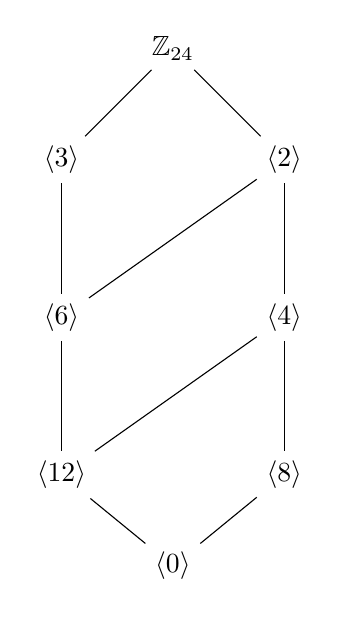
\begin{tikzpicture}[node distance=2cm]
\node(Z24)                           {$\Z_{24}$};
\node(2Z)       [below right of=Z24] {$\left<2\right>$};
\node(3Z)      [below left of=Z24]  {$\left< 3 \right>$};
\node(4Z)      [below of=2Z]       {$\left< 4 \right>$};
\node(8Z)      [below of=4Z]       {$\left< 8 \right>$};
\node(6Z)      [below of=3Z]      {$\left< 6 \right>$};
\node(12Z)		[below of=6Z]		{$\left< 12 \right>$};

\node(1)            [below =6cm of Z24]     {$\left<0\right>$};
\draw(Z24)       -- (2Z);
\draw(Z24)       -- (3Z);
\draw(3Z)      -- (6Z);
\draw(6Z)      --  (12Z);
\draw(2Z)       -- (6Z);
\draw(2Z)       -- (4Z);
\draw(4Z)       -- (8Z);
\draw(8Z)      -- (1);
\draw(12Z)      -- (1);
\draw(4Z)      --  (12Z);
\end{tikzpicture}
\end{figure}

\textbf{($\Z_{36}$)}. Note $|\Z_{36}|=36$ and $\left< 1 \right>=\Z_{36}$. By corollary 3.5.4(b), if $H$ is a subgroup of $\Z_{36}$ then  $H=\left< k \right>$ for some divisor of $36$. So the subgroups of $\Z_{36}$ are $\left< 1 \right>, \left< 2 \right>, \left< 3 \right>, \left< 4 \right>, \left< 6 \right>, \left< 9 \right>, \left< 12 \right>, \left< 18 \right>$. Also, 36 divides itself so $ \left< 36 \right>=\left< 0 \right>$ is a subgroup of $\Z_{36}$. Next by corollary 3.5.4(c) since $3|6$, $6|12$, and $12 | 36$; $3|6$, $6|18$, $18|36$; $3|9$, $9|18$, $18|36$; $2|4$, $4 | 12$, $12 | 36$; $2|6$, $6| 12$, $12 | 36$; and $2 |6$, $6|12$, and $12 | 24$ we must have the following containments: $
\left< 3 \right> \supseteq \left< 6 \right> \supseteq \left< 18 \right>\supseteq \left< 0 \right>; \left< 3 \right> \supseteq \left< 6 \right> \supseteq \left< 12 \right>\supseteq \left< 0 \right>; \left< 3 \right> \supseteq \left< 9 \right> \supseteq \left< 18 \right>\supseteq \left< 0 \right>; \   \left< 2 \right>\supseteq \left< 4 \right>\supseteq \left< 12 \right>\supseteq \left< 0\right>; \left< 2 \right>\supseteq \left< 6 \right>\supseteq \left< 12 \right>\supseteq \left< 0 \right>; \text{ and } \left< 2 \right>\supseteq \left< 6 \right>\supseteq \left< 18 \right>\supseteq \left< 0 \right>
$
Therefore we have the following subgroup diagram:
\\

\begin{figure}[H]
\centering
\begin{tikzpicture}[node distance=2cm]
\node(Z36)                           {$\Z_{36}$};
\node(2Z)       [below left of=Z24] {$\left<2\right>$};
\node(3Z)      [below right of=Z24]  {$\left< 3 \right>$};
\node(4Z)      [below left of=2Z]       {$\left< 4 \right>$};
\node(9Z)      [below right of=3Z]       {$\left< 9 \right>$};
\node(6Z)      [below left of=3Z]      {$\left< 6 \right>$};
\node(12Z)		[below left of=6Z]		{$\left< 12 \right>$};
\node(18Z)		[below right of =6Z] {$\left< 18 \right>$};

\node(1)            [below =5cm of Z36]     {$\left<0\right>$};
\draw(Z36)       -- (2Z);
\draw(Z36)       -- (3Z);
\draw(3Z)      -- (6Z);
\draw(3Z)      -- (9Z);
\draw(9Z)      -- (18Z);
\draw(6Z)      --  (12Z);
\draw(6Z)      --  (18Z);
\draw(2Z)      --  (6Z);
\draw(18Z)      --  (1);
\draw(2Z)       -- (4Z);
\draw(4Z)       -- (12Z);
\draw(12Z)      -- (1);
\end{tikzpicture}
\end{figure}

\begin{homeworkProblem}[Exercise 3.5.13: Show that in a finite cyclic group of order $n$, the equation $x^m=e$ has exactly $m$ solutions, for each positive integer $m$ that is a divisor of $n$.]
\begin{proof}
 	By theorem 3.5.2, since $|G|=n$ and $G$ is cyclic, $G \cong \Z_n$. So, we will work in $\Z_n$. If $x^m=e$ in $\Z_n$, then $[mx]_n=[0]_n$. Assume $m|n$. Then, $n=dm$ for some $d \in \Z, \ d \neq 0$. To show there exists exactly $m$ such $x \in \Z_n$, we will show $\{[x]_n : [mx]_n=[0]_n\}=\{[kd]_n \ : \ k \in \Z_m\}$. Let $y \in \{[x]_n : [mx]_n=[0]_n\}$ so $0 \leq y < n$. Then, $my \equiv 0 \MOD n)$ which implies $my=ln$. Let $l$ be the smallest positive integer such that $my=ln$. Since $n=dm$ we have $my=ldm$ and so $y=ld$. Since $0\leq y < n$, $0 \leq my < mn$ and $0 \leq my < mdm$. Further $0 \leq y < dm$. Since $y=ld$ we have $0 \leq ld < dm$ so $0 \leq l < m$. Thus, $y=ld$ for $l \in \Z_m$ which implies $y \in \{[kd]_n \ : \ k \in \Z_m\}$. \\
 	Next, suppose $y \in \{[kd]_n \ : \ k \in \Z_m\}$. Then, $y\equiv kd \MOD n)$ for $0 \leq k < m$. Equivalently, $my\equiv mkd \MOD n)$ so $my\equiv k(dm) \MOD n)$. Sine $k(dm)=k(n)$ and $k(n) \equiv 0 \MOD n)$ we have $my\equiv 0 \MOD n)$. Thus, $y \in \{[x]_n : [mx]_n=[0]_n\}$. \\
 	Hence, $\{[x]_n : [mx]_n=[0]_n\}=\{[kd]_n \ : \ k \in \Z_m\}$. We claim the number of elements in $\{[kd]_n \ : \ k \in \Z_m\}$ is $m$. If there weren't $m$ elements then there must exists some $k_1, k_2 \in \Z_m$ such that $k_1d \equiv k_2d \MOD n)$, but $k_1 \not \equiv k_2 \MOD m)$. Thus, $k_1d = k_2d + bn$ for some $b \in \Z$. Therefore, $k_1d=k_2d+b(dm)$ so $k_1 = k_2 + bm$ which implies $k_1 \equiv k_2 \MOD m)$. Thus, there are $m$ elements in the set $\{[kd]_n \ : \ k \in \Z_m\}$ which is equal to the set $\{[x]_n : [mx]_n=[0]_n\}$. Thus, there are exactly $m$ integers such that $mx \equiv 0 \MOD n)$. Therefore, since $G \cong \Z_n$, the equation $x^m=e$ has exactly $m$ solutions for each positive integer $m$ that is divisor of $n$. 
 	\end{proof}
\end{homeworkProblem}


\begin{homeworkProblem}[Exercise 3.5.16: Let $G$ be any group with no proper, nontrivial subgroups, and assume that $|G|>1$. Prove that $G$ must be isomorphic to $\Z_p$ for some prime $p$.]
\begin{proof}
Let $G$ be any group with no proper, nontrivial subgroups, and assume that $|G|>1$. Then, $|G| \geq 2$ so $G$ contains an identity element, $e$, and some other element $g \neq e$. By proposition 3.2.6(a), $\left< g \right>$ is a subgroup of $G$. Since $G$ has no proper, nontrivial subgroups, and because $g\neq e$, $\left< g \right>=G$. Thus, $G$ is cyclic. Suppose $|G|= \infty$. Then, by theorem 3.5.2(a), $G \cong \Z$. However, from page 136 of Beachy, we know $\Z$ has proper subgroups of the form $m\Z$ with $m \in \Z$. Since $G$ has no proper subgroups, $G \not \cong \Z$ and so $|G|\neq \infty$. Thus, $|G|=n$. So $G$ is a finite cyclic group. On page 136 of Beachy, we know if $G=\left< g \right>$ is a finite cyclic group, then for every positive divisor $m$ of $n$, $\left< g ^m \right>$ is a subgroup of $G$. If $m\neq 1$ and $m\neq n$, then $\gcd(m,n)=m$ and by proposition 3.5.3, $|\left< g ^m \right>|=\frac{n}{m}<n$. Thus, if $m\neq 1$ and $m\neq n$, $\left< g ^m \right>$ is a proper subgroup of $G$. Since $G$ does not have proper subgroups, this contradiction implies, $m=1$ or $m=n$. Hence, $1,n$ are the only divisors of $n$ which implies $n=p$ for some prime number $p$. Then, by theorem 3.5.2, $G \cong \Z_p$ for some prime $p$. 
\end{proof}
\end{homeworkProblem}


\begin{homeworkProblem}[Exercise 3.5.18: Prove that $\sum_{d|n}\varphi(d)=n$ for any positive integer $n$.]
\begin{proof}
Suppose $n$ has $N$ divisors. Then, rewrite $\sum_{d|n}\varphi(d)=\sum_{k=1}^N\varphi(d_k)$ where all $d_k | n$ are considered. Consider some cyclic group $G = \left< g \right>$ with $|G|=n$. By Theorem 4(5) of Boyton (Cyclic Group handout), for every divisor $d_k$ of $n$, $G$ has exactly one subgroup of order $d_k$. Additionally, by Theorem 4(4) of Boyton, every subgroup of $G$ can be as $\left< g^d \right>$ for some $d | n$. Thus, consider the collection $\{H_k \leq G :  H_k=\left< g^{d_k} \right>, |H_k|=d_k \}_{k=1}^N$. Define $\sim$ on $G$ where $a\sim b$ if and only if $\left<a \right> = \left< b \right>$. By lemma 0.1 below, we know $\sim$ defines an equivalence relation. Let $A_k$ be the equivalence class of $H_k$. Then, $A_k$ contains all generators of $H_k$. From Theorem 4(3) of Boyton, we know $g^s$ generates $H_k$, $|H_k|=d_k$ if and only if $\gcd(s,d_k)=1$. Thus, $H_k$ has $\varphi(d_k)$ possible generators. So $|A_k|=\varphi(d_k)$. Since $A_k$ are equivalence classes, $A_k \cap A_j=\O$ for all $k\neq j$. By lemma 0.2 below, $G=\bigsqcup_{k=1}^N A_k$; therefore, $|G|=|\bigsqcup_{k=1}^N A_k|$. Since $\bigsqcup_{k=1}^N A_k$ is a disjoint union, $|\bigsqcup_{k=1}^N A_k|= \sum_{k=1}^N |A_k|= \sum_{k=1}^N \varphi(d_k)$. Also, $|G|=n$, so $\sum_{k=1}^N \varphi(d_k)=n$. 
\begin{lemma}
Define $\sim$ on $G$ where $a\sim b$ if and only if $\left<a \right> = \left< b \right>$. Then, $\sim$ is an equivalence relation.	
\begin{proof}
\textbf{(reflexive)} For any element $a \in G$, $\left<a \right> = \left< a \right>$, so $a\sim a$.\\
\textbf{(symmetric)} For any $a,b \in G$, if $a \sim b$, then $\left<a \right> = \left< b \right>$. Thus, $\left< b \right> = \left< a \right>$ so $b \sim a$.
\textbf{(transitive)} Suppose for $a,b,c \in G$, $a\sim b$ and $b \sim c$. Then, $\left<a \right> = \left< b \right>$ and $\left<b \right> = \left< c \right>$ so $\left<a \right> = \left< c \right>$. Thus, $a \sim c$. 
\end{proof}
\end{lemma}
\begin{lemma}
$G=\bigsqcup_{k=1}^N A_k$. 
\begin{proof}
First, show $G \subseteq \bigsqcup_{k=1}^N A_k$. Let $g \in G$. Then $\left< g\right> \leq G$ and since $1 | n$ we have $\left< g\right> \in \{H_k \leq G :  H_k=\left< a^{d_k} \right>, |H_k|=d_k \}_{k=1}^N$. Thus, $\left< g \right> = H_1 = A_1$ Thus, $g \in \bigsqcup_{k=1}^N A_k$. \\
Next, show $G \supseteq \bigsqcup_{k=1}^N A_k$. Let $a \in \bigsqcup_{k=1}^N A_k $. Then $a \in A_k$ for some $k$. For all $k$, $A_k \leq G$, so $a \in G$.
\end{proof}	
\end{lemma}


\end{proof}
\end{homeworkProblem}
\begin{homeworkProblem}[Exercise 3.5.19: Let $n=2^k$ for $k>2$. Prove that $\Z_n^\times$ is not cyclic. ]
\begin{proof}
Let $n=2^k$ for $k>2$. Then, $|\Z_n^\times|=2^k>4$. Notice $n>4$ implies $\frac{n}{2}+1 > 1$ and $\frac{n}{2}-1 > 1$ as well as: \[
n+4<n+n=2n; \quad n<2n-4; \quad \frac{n}{2}<n-2; \quad \frac{n}{2}+1<n-1 \text{ and similarly, } \frac{n}{2}<n; \quad \frac{n}{2}-1<n-1.
\]
Thus, $1, \frac{n}{2}\pm 1 \in \Z_n^\times$. Notice $\frac{n}{2}\pm 1, n-1$ have order 2 in $\Z_n^\times$:
\[
\begin{array}{rrrr}
	(\frac{n}{2}+1)^2 & \equiv \left(\frac{2^k}{2}\right)^2 + 2\left(\frac{2^k}{2}\right) + 1 & \equiv 2^k2^{k-1}+2^k+1 & \equiv 1 \MOD n)\\
	(\frac{n}{2}-1)^2 & \equiv \left(\frac{2^k}{2}\right)^2 - 2\left(\frac{2^k}{2}\right) + 1 & \equiv 2^k2^{k-1}-2^k+1 & \equiv 1 \MOD n)\\
	& (n-1)^2 & \equiv n^2-2n+1 & \equiv 1 \MOD n)\\
\end{array}
\]
Because $n>4$, $1 \neq \frac{n}{2}+ 1 \neq \frac{n}{2} - 1 \neq n-1$. From above, we know in $\Z_n^\times$, $o(\frac{n}{2}+ 1) = o(\frac{n}{2} - 1) = o(n-1)=2$. So we have three distinct elements of order 2. Suppose $\Z_n^{\times}$ is cyclic. Then, by theorem 3.5.2(b), $\Z_n^\times \cong \Z_n$. Since $\Z_n^\times$ has even order, $|\Z_n|=2l$ for some $l \in \Z^+$. However, by the lemma below, $\Z_n$ has exactly one element of order 2 where $\Z_n^\times$ has at least three. By proposition 3.4.3, isomorphisms preserve order. Thus, $\Z_n^\times \not \cong \Z_n$ which implies $\Z_n^\times$ is not cyclic. 
\begin{lemma}
	$\Z_{2l}$ has exactly one element of order 2.
\end{lemma}
 \begin{proof} Note $l$ is an element of order 2: $l + l \equiv 0 \MOD 2l)$. If there exists $g \in \Z_{2l}$ with $l \neq g$ and $g \neq 0$ (since 0 has order 1) such that $2g \equiv 0 \MOD 2l)$. Then $g \equiv 0 \MOD l$ implies $g=hl$ for some $h\in \Z$. But, $g \in \Z_{2l}$ so $0 < g < 2l$ and so $0 < hl < 2l$ implies $0 < h < 2$ so $h=1$ and $l=g$. Thus, there exists exactly one element of order 2 in $\Z_{2l}$. 
 \end{proof}

\end{proof}

\end{homeworkProblem}

\begin{homeworkProblem}[Exercise 3.5.20: Let $G$ be a group with $p^k$ elements, where $p$ is a prime number and $k \geq 1$. Prove that $G$ has a subgroup of order $p$. ]
\begin{proof}
Let $G$ be a group with $p^k$ elements, where $p$ is a prime number and $k \geq 1$. Then, $|G|=p^k$. By Lagrange's Theorem, the order of any element in $G$ must divide the order of $G$. So for any $g \in G$ with $g \neq e$, $|g|=p^l$ for $1 \leq l \leq k$.  If $|g|=p$, then $\left< g \right>$ is a subgroup of $G$ of order $p$. If $|g|=p^l$ for $2 \leq p \leq k$, then consider $h=g^{p^{l-1}}$. Since ${p^l}$ is the smallest integer, $t$, such that $g^{t}=e$, $p^{l-1}< p^l$ implies $g^{p^{l-1}}\neq e$. Notice $h=(g^p)^{l-1}=(g^{p^lp^{-1}})=(g^{p^l})^{p^{-1}}=e^{p^{-1}}=e^{-p}$. Therefore $h^p=(e^{-p})^p=e^{\frac{1}{p}\cdot p}=e^1=e$. So the order of $h$ must divide $p$. Since $h \neq e$, $|h|=p$ so $\left< h \right>$ is a subgroup of $G$ of order $p$. 
\end{proof}

\end{homeworkProblem}

\end{flushleft}
\end{spacing}
\end{document}

%%%%%%%%%%%%%%%%%%%%%%%%%%%%%%%%%%%%%%%%%%%%%%%%%%%%%%%%%%%%%

%----------------------------------------------------------------------%
% The following is copyright and licensing information for
% redistribution of this LaTeX source code; it also includes a liability
% statement. If this source code is not being redistributed to others,
% it may be omitted. It has no effect on the function of the above code.
%----------------------------------------------------------------------%
% Copyright (c) 2007, 2008, 2009, 2010, 2011 by Theodore P. Pavlic
%
% Unless otherwise expressly stated, this work is licensed under the
% Creative Commons Attribution-Noncommercial 3.0 United States License. To
% view a copy of this license, visit
% http://creativecommons.org/licenses/by-nc/3.0/us/ or send a letter to
% Creative Commons, 171 Second Street, Suite 300, San Francisco,
% California, 94105, USA.
%
% THE SOFTWARE IS PROVIDED "AS IS", WITHOUT WARRANTY OF ANY KIND, EXPRESS
% OR IMPLIED, INCLUDING BUT NOT LIMITED TO THE WARRANTIES OF
% MERCHANTABILITY, FITNESS FOR A PARTICULAR PURPOSE AND NONINFRINGEMENT.
% IN NO EVENT SHALL THE AUTHORS OR COPYRIGHT HOLDERS BE LIABLE FOR ANY
% CLAIM, DAMAGES OR OTHER LIABILITY, WHETHER IN AN ACTION OF CONTRACT,
% TORT OR OTHERWISE, ARISING FROM, OUT OF OR IN CONNECTION WITH THE
% SOFTWARE OR THE USE OR OTHER DEALINGS IN THE SOFTWARE.
%----------------------------------------------------------------------%
